\documentclass[preprint,12pt]{elsarticle}

% Basic packages
\usepackage[a4paper, margin=1in]{geometry}
\usepackage{graphicx}
\usepackage{amsmath}
\usepackage{hyperref}
\usepackage{longtable}
\usepackage{booktabs}
\usepackage{caption}
\usepackage{subcaption}
\usepackage{overpic}
\captionsetup[table]{skip=10pt}

% Add Unicode support
\usepackage[utf8]{inputenc}
\usepackage[T1]{fontenc}
\usepackage{textcomp}

% Add color support
\usepackage{xcolor}

% Line numbering
\usepackage{lineno}
\leftlinenumbers
\renewcommand\linenumberfont{\normalfont\small\color{gray}}

% Add support for text formatting
\usepackage{array}
\usepackage{enumitem}
\usepackage{float}

% Add support for special characters
\usepackage{textcomp}
\usepackage{gensymb}


% Citas en texto tipo APA (p.ej., \citep{key} -> (Gonzales et al., 2023))
\biboptions{authoryear,round,semicolon}

%-----------------------------------------------
% METADATA
\title{Predicting plant diversity facets from Landsat phenology and topography in central and southern Chile}

\author[1,2,3]{Javier Lopatin\corref{cor1}}
\ead{javier.lopatin@uai.cl}

\author[4]{Rocío Araya-López}
\ead{ro.arayalopez@gmail.com}

\author[2,5]{Dylan Craven}
\ead{dylan.craven@umayor.cl}

\address[1]{Center for Earth and Space, Faculty of Engineering and Science, Adolfo Ibáñez University, Av. Diagonal Las Torres 2460, Santiago, Chile, 7941169}

\address[2]{Data Observatory Foundation, ANID Technology Center No. DO210001, Santiago, Chile, 7510277}

\address[3]{Center for Climate Resilience Research (CR)2, University of Chile, Santiago, Chile, 8370449}

\address[4]{Deakin  Marine Research and Innovation Centre, School of Life and Environmental Sciences, Deakin University, Burwood Campus, Burwood, VIC 3125, Australia}

\address[5]{GEMA Center for Genomics, Ecology and the Environment, Universidad Mayor, Santiago, Chile}

% AGREGAR CORRESPONDING AUTHOR CON COR1
\cortext[cor1]{Corresponding author; javier.lopatin@uai.cl}

%-----------------------------------------------
\begin{document}
\begin{frontmatter}

\begin{abstract}

\end{abstract}

\begin{keyword}

\end{keyword}

\end{frontmatter}

\linenumbers

\section{Introduction}

Biodiversity is not a single number. The number of species in a place, the singularity of
its species composition and the depth of evolutionary history it holds respond to different
processes and imply different conservation decisions, and no one of them substitutes for
the others. Policy frameworks that define which biodiversity variables satellites should
observe list several of these facets side by side \citep{skidmore2021priority}, and two
decades of work have argued that remote sensing can contribute to more than one of them
\citep{wang2019remote,cavenderbares2022integrating}. Yet the maps that reach ecologists are
almost always maps of one facet, derived from one date, and validated in a way that
flatters them. A map of species richness does not say whether a site is compositionally
unique, and neither map says whether the site conserves deep lineages.

Most of that work rests on the spectral variation hypothesis, which treats the spectral
heterogeneity of a pixel neighbourhood as a proxy for habitat heterogeneity and hence for
species diversity. After twenty years the evidence remains inconsistent between ecosystems
\citep{torresani2024reviewing,fassnacht2022about}, and the relationship changes sign
between landscapes \citep{schmidtlein2017the}. Reviews converge on four contextual factors
behind that inconsistency: vegetation type, spatial scale and sensor resolution, the metric
chosen, and changes in reflectance through time caused by phenology
\citep{lenormand2025spectral}. The empirical record matches. Single-date indices from
Landsat and Sentinel-2 explain very little of grassland richness in southern Africa, and a
recent multi-ecosystem assessment concludes that existing remote-sensing models of plant
alpha diversity typically achieve low accuracy \citep{wang2026plant}. The hypothesis works
where diversity is low \citep{hayden2024highresolution} and weakens as richness rises, when
many species come to share the same spectral space \citep{donnini2024spectral}. Phenology,
in this framing, is a nuisance to be controlled.

The alternative is to treat the temporal trajectory as the signal. Land surface phenology
integrates community dynamics from species to region \citep{dronova2022remote}; plant
diversity measurably damps interannual phenological variability across wetlands at national
scale \citep{dronova2022plant}; and functional diversity itself varies through the season
and does so differently between biomes, which makes any single date insufficient by
construction \citep{mederer2025unraveling}. Spectral asynchrony among pixels has been
proposed as a measure of ecosystem response diversity \citep{mazzochini2024spectral}, and
clustering MODIS time series over more than 23,000 cells recovers both alpha and beta
gradients in France \citep{lenormand2025spectral}. Working in grasslands over two
consecutive years, \citet{gholizadeh2020multitemporal} state the omission plainly: the
temporal dynamics of plant communities have been overlooked in many studies of remotely
sensed diversity. Our own earlier work ties the mechanism to communities, showing that
interannual variability of satellite phenology relates to plant community composition
\citep{lopatin2023interannual,lopatin2026remotely}. What is missing is the step from
phenology as a correlate to phenology as the input of a predictive model of several facets
at once.

That step matters because of where large-scale biodiversity maps currently stand. The
models that cover continents or the globe are built from vegetation-plot databases and
climatic predictors rather than from satellite time series, and their honest accuracies are
modest: global maps of vascular plant alpha diversity trained on 170,272 plots reach a
Pearson correlation of 0.49 under spatially constrained block cross-validation
\citep{sabatini2022global}, and global machine-learning models of species and phylogenetic
richness explain 70.3\% and 73.7\% of the variance under spatial cross-validation, against
80.9\% and 83.3\% under random cross-validation, at a grain of thousands of square
kilometres \citep{cai2023global}. Random Forest models of European forest alpha diversity
built on 73,134 plots explain 51 to 71\% \citep{vecera2019alpha}. Where satellite
predictors do carry the model, the extent collapses to landscapes: the best recent
comparison of spaceborne sensors for tree species diversity reports a mean $R^2$ of 0.48
over 4,000\,km$^2$ \citep{liu2024tree}. We found no national or continental map of plant
diversity facets built from satellite time series and validated against field plots, and
the imbalance is documented from the other side: remote sensing is used in Latin America
and the Caribbean far below what the region's biodiversity would warrant
\citep{garzonlopez2024remote}.

The accuracies that are published cannot be taken at face value either. Random
cross-validation over spatially clustered training data rewards interpolation: across 43
deep-learning architectures applied to satellite time series, random splitting inflates
performance by 16 to 25 percentage points relative to spatially independent validation
\citep{arrudabruno2026deep}, and mapping accuracy elsewhere falls from 70--79\% under
cross-validation to 44--56\% against independent data \citep{maynard2019ecological}. Global
models further extrapolate beyond the environments they were trained in, and predictions
outside the area of applicability should be avoided altogether
\citep{meyer2022machine,ludwig2023assessing,ploton2020spatial}. Transfer through time is
tested least of all, although the evidence that exists is discouraging: the relationship
between field and spectral diversity weakened between two consecutive years in the same
grassland \citep{gholizadeh2020multitemporal}, and extrapolating trait models to new
seasons drops $R^2$ to between 0.15 and 0.42 \citep{ji2024leaf}. A model intended to produce
a time series of maps has to be judged on exactly this axis.

Chile offers an unusually clean test. Its Mediterranean and temperate vegetation spans 25
degrees of latitude and is nearly absent from this literature, and the regional precedents
are single-date, single-facet studies of species richness
\citep{ceballos2015comparison,lopatin2016comparing}. Two recent plot networks change what
is possible: Parcelas-CL, a community-sourced vegetation database
\citep{cerdaparedes2026parcelascl}, and a national forest inventory of tree-level records,
which together provide 3,102 plots between 30 and 55\textdegree{}S, each with its own census
year. Because Landsat covers the full census period, every plot can be paired with the
phenology of the three years that ended when it was surveyed, rather than with a single
common image.

We use that design to ask three questions. First, does the raw three-year phenological
trajectory of the pixel containing a plot predict coverage-standardised taxonomic and
phylogenetic richness and the local contribution to beta diversity, and which of these
facets carries signal at all? Second, does the representation matter: does folding the
series into an image and reading it with a convolutional network beat a Random Forest given
the same information, and does self-supervised pretraining help at this sample size?
Third, and most consequential for mapping, does whatever skill exists survive when the
model must predict in spatial blocks it has never seen and in census periods it has never
seen? We answer them with four model families under one design, two cross-validation
schemes, and a deliberate refusal to report the optimistic one alone.

\section{Methods}

\subsection{Study region and vegetation plot networks}

We combined two vegetation plot networks that together span the Mediterranean, temperate
and sub-Antarctic forests and shrublands of Chile between 30\textdegree{}S and
55\textdegree{}S (Fig.~\ref{fig:coverage}). Parcelas-CL is a community-sourced database of
georeferenced vegetation plots contributed by twelve research groups
\citep{cerdaparedes2026parcelascl,zenodo2026parcelascl}. From its 1,485 plots we retained
the subset that a pixel-based model can use: plots with a known census year (1,443),
located between 30\textdegree{}S and 38\textdegree{}S (1,254), censused in the Landsat era
(year $\geq$ 1999; 1,253) and carrying a unique coordinate (1,082). The last filter removed
one contributor's 1999 campaign, in which 160 plots shared eight site-level coordinates and
would have produced identical predictor vectors with different labels. The retained
Parcelas-CL plots were censused between 2003 and 2026 and cover 78.5 to 10,000\,m$^2$
(median 314\,m$^2$).

Living Trees Chile \citep{livingtrees_chile} is a forest inventory that records every tree
(species, diameter at breast height and height) on fixed plots of 250 or 500\,m$^2$
(median 500\,m$^2$) established between 2011 and 2020. We treated the plot coordinate, not
the field sampling-unit code, as the plot identity, because 78 codes repeated across
regions and two coordinates carried two codes each. This yielded 2,021 sites, of which
2,020 contained at least one identified tree species. Living Trees Chile extends the
geographic footprint of the analysis from 30.6\textdegree{}S to 55.0\textdegree{}S. Because
the inventory records trees only, species richness on these plots is tree-species richness
(76 species over the network), whereas Parcelas-CL contributors recorded all woody species
(221 species in the subset used here); we return to this asymmetry in the Discussion.

We merged both networks into a unified pool of 3,102 plots. We prefixed plot identifiers by
source so that the two identifier schemes cannot collide, and we projected all coordinates
onto a Lambert azimuthal equal-area projection centred on Chile (35\textdegree{}S,
71\textdegree{}W), because the UTM~19S grid native to Parcelas-CL distorts distances
strongly near Magallanes. We harmonised species names to the Parcelas-CL taxonomy and
assigned families from the V.PhyloMaker2 family table \citep{jinqian2022vphylomaker2},
adding manual family assignments for genera absent from that table. Throughout the
pipeline every plot keeps exactly one row: facets that an estimator cannot compute for a
plot are stored as missing values and handled by masked losses (Section~\ref{sec:training}),
never by dropping or imputing the plot.

\begin{figure}[tbp]
\centering
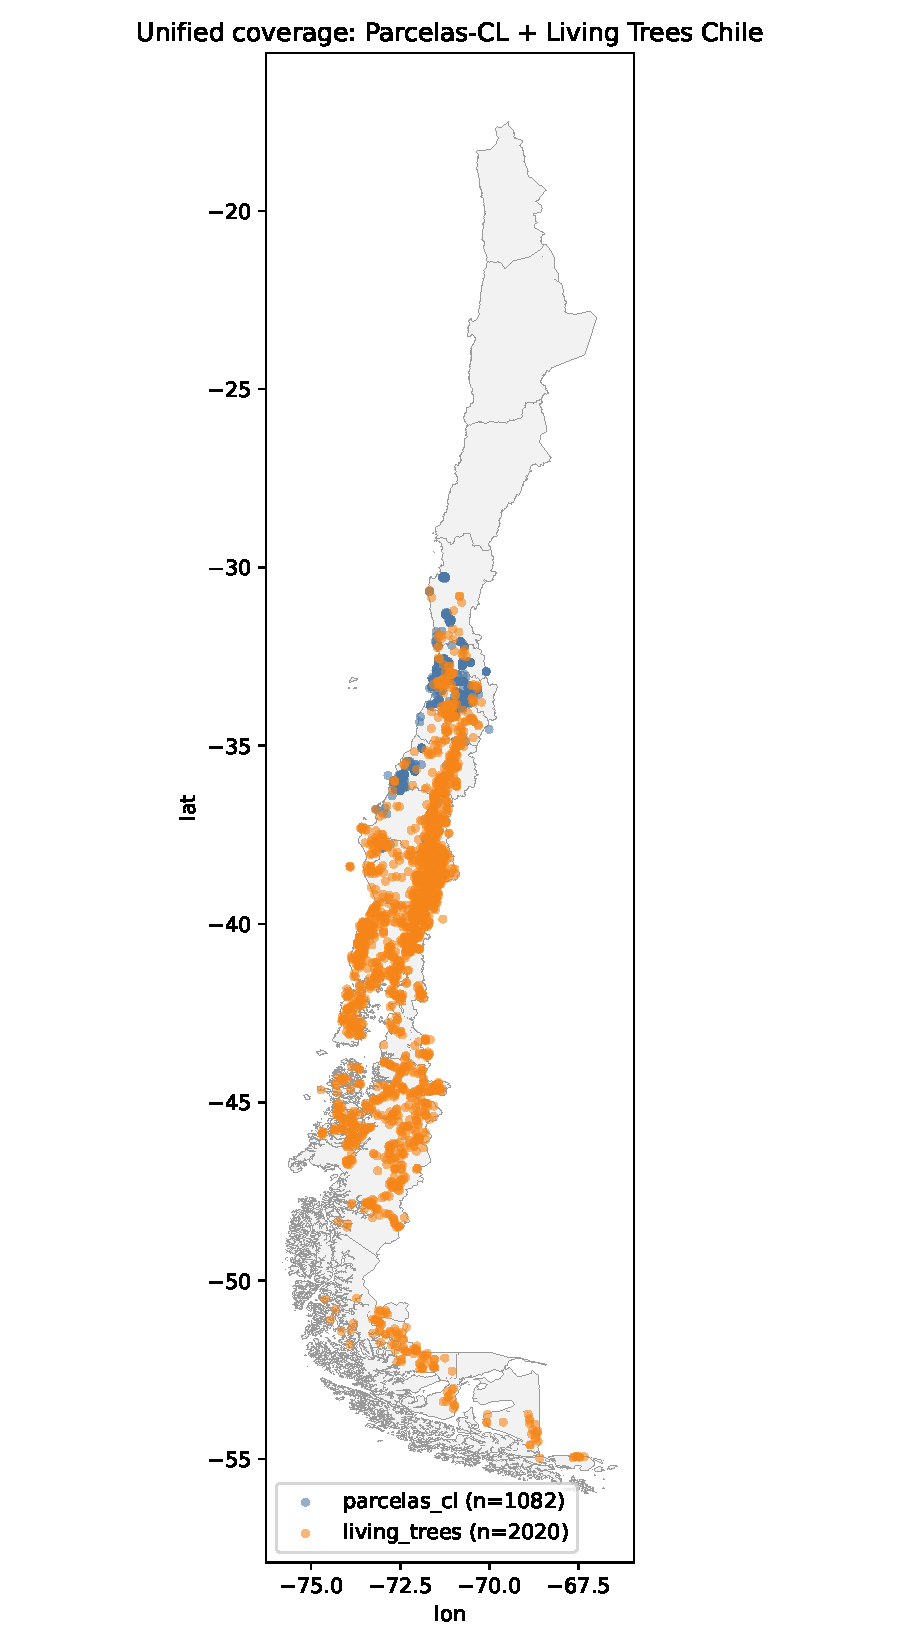
\includegraphics[height=0.62\textheight]{../results/figures/fig19_unified_coverage_map.pdf}
\caption{Geographic coverage of the unified plot pool: 1,082 Parcelas-CL plots
(30--38\textdegree{}S) and 2,020 Living Trees Chile plots (30.6--55.0\textdegree{}S).}
\label{fig:coverage}
\end{figure}

\subsection{Diversity facets}
\label{sec:facets}

We computed three families of diversity facets on the subset of the unified pool that
carries genuine counts of individuals, following the estimators that
\citet{perezgiraldo2026environmental} applied to Andean plots: 479 Parcelas-CL plots whose
contributors recorded the number of individuals per species, and the 2,020 Living Trees
plots, for which we counted tree stems per species. This count-based pool holds 2,499 plots
and 261 species, with a median of five species per plot in Parcelas-CL and three in Living
Trees. We excluded the Parcelas-CL cover and basal-area strata from these facets because
the coverage-based estimators below require abundances that behave like counts.

\paragraph{Local contribution to beta diversity.}
We quantified the compositional uniqueness of each plot as its local contribution to beta
diversity (LCBD; \citealp{legendre2013beta}). We computed the percentage-difference
dissimilarity between plots, which is the quantitative form of the S{\o}rensen index in the
Podani family \citep{podani2011new,podani2013general}, with the R package
\emph{adespatial} \citep{legendre2014interpreting,dray2023adespatial}, took its square root
to make the dissimilarity Euclidean, and derived the LCBD of each plot from that matrix.
LCBD values sum to one over the 2,499 plots of the count pool; we refer to this facet as
LCBD.

\paragraph{Coverage-standardised taxonomic and phylogenetic diversity.}
We expressed taxonomic diversity (TD) and phylogenetic diversity (PD) as Hill numbers of
order $q = 0$, 1 and 2 \citep{hill1973diversity,chao2014unifying}, standardised by sample
coverage rather than by sample size \citep{chao2012coverage,chao2014rarefaction}, with the
R package \emph{iNEXT.3D} \citep{chao2021measuring}. We estimated the three orders
separately for each plot from its abundance counts, without bootstrap replicates, at the
sample coverage that the plot's own sample reaches when extrapolated to twice its size.
Each plot was therefore standardised to its own maximum reliable coverage rather than to a
common level across plots; this coverage was high but variable (median 0.99, range
0.53--1.00). The estimator requires at least five observed species per assemblage, which
restricted TD to 895 plots (244 Parcelas-CL, 651 Living Trees). For PD we used the
phylogeny pruned to the species of each plot and expressed the result as the effective
number of equally divergent lineages, with the depth of the pruned subtree as the
reference time. PD also requires that species be
present in the phylogeny, which restricted it to 888 plots (237 Parcelas-CL, 651 Living
Trees). We denote these facets TD$_q$ and PD$_q$.

\paragraph{Phylogeny.}
We built the phylogeny with V.PhyloMaker2 \citep{jinqian2022vphylomaker2} from the
GBOTB.extended.TPL megatree, which combines the seed-plant backbone of
\citet{smithbrown2018constructing} with the tree of \citet{zanne2014three}, using scenario
S3 to graft species absent from the megatree at the midpoint of their genus branch. The
unified species list yielded a tree of 610 tips, 55\% of which occupy their own position in
the megatree and 45\% of which were grafted by genus.

We re-indexed all seven facets onto the full 3,102-plot pool, leaving missing values where
an estimator did not reach its species floor or where a plot lay outside the count pool
(Table~\ref{tab:facets}).

\begin{table}[t]
\centering
\footnotesize
\caption{Diversity facets modelled in this study, computed on the count-based pool and
re-indexed onto the 3,102-plot unified pool. $n$ is the number of plots with a value, split
into Parcelas-CL (PCL) and Living Trees (LT). LCBD values are multiplied by $10^{4}$.}
\label{tab:facets}
\begin{tabular}{llrrrr}
\toprule
Facet & Estimator & $n$ & PCL / LT & Median & Range \\
\midrule
LCBD & percentage difference (\emph{adespatial}) & 2,499 & 479 / 2,020 & 3.99 & 3.43--4.41 \\
PD$_0$ & coverage-standardised (\emph{iNEXT.3D}) & 888 & 237 / 651 & 4.79 & 2.37--26.6 \\
PD$_1$ & & 888 & 237 / 651 & 2.83 & 1.13--9.08 \\
PD$_2$ & & 888 & 237 / 651 & 2.27 & 1.04--6.11 \\
TD$_0$ & coverage-standardised (\emph{iNEXT.3D}) & 895 & 244 / 651 & 7.22 & 5.00--84.0 \\
TD$_1$ & & 895 & 244 / 651 & 4.60 & 1.15--28.8 \\
TD$_2$ & & 895 & 244 / 651 & 3.60 & 1.04--14.5 \\
\bottomrule
\end{tabular}
\end{table}

\subsection{Landsat time series and phenological curves}
\label{sec:curves}

We extracted Landsat Collection~2 Level-2 surface reflectance \citep{crawford2023landsat}
from Landsat~5, 7, 8 and 9 through Data Cube Chile
\citep{datacubechile,killough2018odc} for the 30-m pixel that contains each plot, on a
UTM~19S grid. For every plot we used a causal three-year
window that ends in the census year ($y-2$ to $y$), so that no observation postdates the
census and the same window definition applies to plots censused in any year. We scaled
digital numbers to reflectance ($\rho = \mathrm{DN} \times 2.75 \times 10^{-5} - 0.2$) and
masked no-data, cloud, cloud shadow, cirrus, dilated cloud and high-confidence snow with
the pixel-quality band of each product before concatenating sensors. We stored every
clear observation with its acquisition date rather than a fitted curve, which lets any
curve construction be revisited without returning to the data cube. Parcelas-CL windows
held between 80 and 265 observation dates per plot; Living Trees windows held a median of
63 clear observations per plot (range 7--186), decreasing southward with cloud cover.

From the red and near-infrared reflectance of each observation we computed the kernel
NDVI \citep{campsvalls2021kndvi}, which saturates less than NDVI over dense canopies:
\begin{equation*}
\mathrm{kNDVI} = \tanh\!\left(\mathrm{NDVI}^2\right), \qquad
\mathrm{NDVI} = \frac{\rho_\mathrm{NIR} - \rho_\mathrm{red}}{\rho_\mathrm{NIR} + \rho_\mathrm{red}}
\end{equation*}
\citep{tucker1979red}. We also tested NDVI, the enhanced vegetation index, the normalised
burn ratio and the soil-adjusted vegetation index as alternative substrates. The five
indices were indistinguishable, with differences smaller than the dispersion between
training runs (Supplementary Section~S1); we retained kNDVI because it is the index of the
pretrained network used to initialise the models and because it gave the highest and most
stable scores on the facet with the strongest signal.

We built the model input as a raw multi-year series rather than as a composite annual
curve. For the pixel that contains each plot we interpolated the clear kNDVI observations
linearly onto 100 equally spaced steps between the first and the last observation of the
window (a step of about 11 days), and smoothed the interpolated series with a five-step
moving mean that shrinks at the series ends. Series with fewer than five clear
observations were left missing. The series remains in calendar time; we applied no phase
rotation. For Living Trees plots we applied the same interpolation to the stored
observation tables.

As an ablation level we also fitted the composite annual curve produced by
\emph{PhenoShape} in the \emph{PhenoSensing} library \citep{lopatin_phenosensing}, which
pools the three years onto a single 52-step day-of-year axis with linear reconstruction and
a five-step moving mean, anchored globally so that the array boundary falls at the regional
trough (day of year 108). The composite averages interannual variation away and carries a
discontinuity at the year boundary, which is why we did not use it in the headline design.

\subsection{Topographic and plot context}
\label{sec:context}

We derived topography from the Copernicus GLO-30 digital elevation model
\citep{esa2022copdem} at 30\,m. We computed the derivatives on a wide neighbourhood and
cropped to the plot window afterwards, so that slope, aspect and curvature are free of edge
effects. The eight variables are elevation, slope, northness and eastness (cosine and sine
of aspect), the heat-load index of \citet{mccune2002heatload} folded about 315\textdegree{}
for the southern hemisphere, the topographic position index \citep{weiss2001topographic}
over a 7$\times$7-pixel neighbourhood, the terrain ruggedness index
\citep{riley1999terrain} and total curvature. We took each variable at the pixel that
contains the plot and added a flag for flat terrain, where the heat-load index is
undefined. We extracted Living Trees topography with the same procedure and joined it to
the plot table by exact coordinate.

To this block we appended the plot area ($\log_{10}$ m$^2$) and indicator variables for
the abundance-recording protocol of the source (cover, individual counts, presence only, or
basal area), because plot area confounds species richness and the protocol indicator
absorbs systematic differences between sources. We imputed missing context values with the
median of the training fold, added a missingness indicator per column, and, for the neural
networks, standardised each column with training-fold statistics
\citep{pedregosa2011scikit}.

\subsection{Predictive models}
\label{sec:models}

We compared four model families under one common design: the kNDVI raw series of the plot
pixel, the context block of Section~\ref{sec:context}, the seven facets as targets (jointly
for the networks, one forest per facet for Random Forest), and the spatial block
cross-validation of Section~\ref{sec:cv}.

\paragraph{Two-dimensional convolutional network.}
We folded the 100-step series into a 10$\times$10 image with a serpentine layout, in which
consecutive rows run in alternating directions so that adjacent cells are always adjacent
in time, following the signal-to-image approach of \citet{lopatin_trait2dcnn}. Each row
spans about 110 days, so a 3$\times$3 kernel reads the series at neighbouring times and
about one season apart. The network (\emph{PhenoNet-S}) is a compact trunk for the
few-thousand-sample regime: a 3$\times$3 stem convolution to 16 channels, four
depthwise-separable 3$\times$3 blocks \citep{chollet2017xception} of 32, 32, 64 and 64
channels, the third with stride 2, each followed by batch normalisation
\citep{ioffe2015batch}, a GELU activation \citep{hendrycks2016gelu} and channel dropout
(0.1), and global average pooling to a 64-dimensional embedding. We concatenated the
context vector to the embedding (late fusion) and mapped it through a two-layer head
(64 units, GELU, dropout 0.3) to the seven outputs. With this input the model has
15,175 parameters.

\paragraph{One-dimensional convolutional network.}
As the control for the second dimension we trained a one-dimensional network with the same
design philosophy (\emph{Pheno1D}): a width-5 stem convolution to 16 channels, four
depthwise-separable width-5 blocks of 32, 32, 64 and 64 channels, the second and third with
stride 2, circular padding along the time axis, global average pooling, and the same
late-fusion head. It has 14,535 parameters.

\paragraph{Random Forest.}
We trained one Random Forest regressor \citep{breiman2001random} per facet with
scikit-learn \citep{pedregosa2011scikit} on the concatenation of the 100 series values and
the context block, with 500 trees, one third of the predictors sampled at each split and a
minimum of two samples per leaf. For each facet we dropped the plots for which that facet
is missing. The Random Forest read the same series and the same context block as the
networks.

\paragraph{Masked-autoencoder initialisation.}
We tested whether self-supervised pretraining helps the two-dimensional network by
initialising its trunk from a convolutional masked autoencoder \citep{he2022masked}. We
pretrained the autoencoder, which uses the \emph{PhenoNet-S} trunk as encoder and a small
convolutional decoder, to inpaint 2$\times$2 patches of the serpentine image with 60\% of
the patches masked, computing the loss on the masked patches only, for 40 epochs with AdamW
(learning rate $10^{-3}$, weight decay $10^{-2}$, cosine schedule, batch size 256). The
pretraining pool consisted of the 27,050 per-pixel composite kNDVI curves of the
Parcelas-CL windows (25 pixels $\times$ 1,082 plots), imaged as 8$\times$8 serpentine
arrays; because global average pooling makes the trunk agnostic to image size, the
pretrained weights transfer to the 10$\times$10 raw-series input. Pretraining saw no
diversity target, but it did see pixels of plots that later fall in test folds. We
therefore report this variant as exploratory and do not treat it as a clean member of the
family comparison.

\subsection{Training protocol}
\label{sec:training}

We implemented and trained the networks in PyTorch \citep{paszke2019pytorch} with a
masked Huber loss \citep{huber1964robust} ($\delta = 1$)
over the seven targets, so that a plot contributes to every facet it carries and to none it
lacks. We transformed each target with a Yeo--Johnson power transformation
\citep{yeo2000new} fitted on the training data and standardised to unit variance, which
also equalises the weight of the facets in the joint loss. We optimised with AdamW
\citep{loshchilov2019decoupled} (learning rate $3 \times 10^{-3}$, weight decay
$10^{-2}$), a ten-epoch linear warm-up followed by cosine decay over at most 300 epochs,
batches of 64 and gradient-norm clipping at 1. We carved a grouped validation split (20\%
of the training fold, grouped by the outer scheme's own grouping variable: spatial blocks
under spatial block cross-validation, census periods under the leave-location-and-time-out
scheme) out of every training fold, stopped training when the validation loss had not improved for 25 epochs
and restored the best weights. The target transformation and the context preprocessing
were fitted on the fitting split only. We augmented the series on the fly before imaging:
a fractional temporal jitter (normal, standard deviation 0.5 step), an amplitude factor
(uniform, $\pm$5\%), a baseline offset (uniform, $\pm$0.02) and Gaussian noise (standard
deviation 0.01). We back-transformed predictions to original units with Duan's smearing
estimator \citep{duan1983smearing}, using the residuals of the validation split for the
networks and the out-of-bag residuals for Random Forest. For Random Forest the target
transformation and the median imputation were fitted on the whole training fold, without
standardisation. We repeated every network configuration with five random seeds and every
Random Forest configuration with three. On one consumer GPU (NVIDIA GeForce RTX 2060) a
five-fold, five-seed network run took 8 to 11 minutes and a five-fold, three-seed Random
Forest run took 114\,s.

\subsection{Cross-validation}
\label{sec:cv}

Random cross-validation over spatially clustered plots rewards spatial interpolation and
overstates transferability \citep{roberts2017crossvalidation,ploton2020spatial}. We
therefore evaluated every model with spatial block cross-validation
\citep{valavi2019blockcv}. We tiled the equal-area projection with 20$\times$20\,km blocks,
which grouped the 3,102 plots into 610 occupied blocks, and assigned whole blocks to five
folds with a grouped $k$-fold that balances plot richness across folds. Every plot was
predicted exactly once from a model that never saw its block; the test folds held 572 to
635 plots. On the Parcelas-CL subset this block size places a test plot at a median
distance of about 12\,km from the nearest training plot, comparable with the 13\,km that
separates a typical native-vegetation pixel from its nearest plot, which is the distance
at which a map would have to predict \citep{linnenbrink2026stemp,meyer2021predicting}.
Because plots of every census year fall in every fold, the held-out blocks span the
2003--2026 census period and the block scores integrate interannual variation in
vegetation and in inventory conditions; what they do not test is extrapolation to years
absent from the training set, which the next scheme addresses.

To test transfer in space and time together we built a leave-location-and-time-out scheme
that crosses the five spatial folds with six census periods (block edges 2002, 2011, 2015,
2018, 2021, 2024 and 2027). Each test cell is one spatial fold in one period; its training
set excludes the whole spatial fold and, in addition, every plot whose own three-year
observation window overlaps the window of the test cell, so that no Landsat observation
is shared between training and test. Twenty-nine cells with at least five test plots covered
the pool, each plot being tested once (9 to 381 test plots per cell, median 69). We report
this scheme as a stringent transferability diagnostic in the sense of the STeMP reporting
protocol \citep{linnenbrink2026stemp}, not as an estimate of map accuracy.

\subsection{Evaluation and design comparisons}
\label{sec:ablations}

We scored every configuration with the coefficient of determination
$R^2 = 1 - \sum(\hat{y}-y)^2/\sum(y-\bar{y})^2$ computed on the out-of-fold predictions of
all plots that carry the facet, in original units, separately for each seed, and we report
the mean over seeds. Negative values mean that the model predicted worse than the training
mean. Because the abundance-weighted facets ($q = 1$, 2) showed no signal under any
configuration, we ranked configurations by the mean $R^2$ over the three facets with usable
signal (LCBD, PD$_0$ and TD$_0$); averaging over all seven facets would have hidden the only
signal present. We report the standard deviation over seeds next to each mean and ran no
inferential tests on these comparisons; we do not interpret differences between
configurations that are smaller than those standard deviations. For completeness we also
computed the $R^2$ of the seed-ensemble prediction (the mean of the seed predictions per
plot), which is the score a deployed ensemble would obtain; we quote it where it differs
materially from the seed mean.

Before the family comparison we fixed the design with two post-hoc screening sweeps under
the two-dimensional network and spatial block cross-validation: the curve format (raw
series or composite curve) and the vegetation index (five alternatives, Supplementary
Section~S1). These sweeps and the family comparison share the same folds,
so the headline scores are conditioned on the screening choices; we did not run a nested
selection audit on the unified pool.

\subsection{Model for mapping}
\label{sec:finalmodel}

For multitemporal map inference we refit the selected configuration on all 3,102 plots.
Spatial block cross-validation is the validation we rely on for this use: its held-out
blocks contain plots censused throughout 2003--2026, so the reported scores already
integrate variation among census years, whereas the leave-location-and-time-out scheme
withholds whole periods and measures extrapolation to unobserved years
(Section~\ref{sec:results_llto}). The refit uses the two-dimensional network with
masked-autoencoder initialisation, the configuration with the highest observed block
cross-validated richness scores, trained on every plot without a validation split for a
fixed budget of 33 epochs, the median of the best epochs (stopping epoch minus the 25-epoch
patience) of five preliminary early-stopped fits, with the same optimiser and schedule as
in Section~\ref{sec:training} and with the target transformation and the context
preprocessing fitted on all plots; five seeds provide checkpoints for ensemble prediction,
and the same ensemble is applied to the Landsat series of every year to produce one map
per year.
% Implemented on the GPU box 2026-09-02: scripts/72 --all-data --epochs 33 (default),
% trainer.train_fixed_epochs; run dir results/models_unified/<RUN_TAG>_alldata/final,
% log logs/81_train_final_map_model_alldata.log. Uncommitted there at the time of writing;
% pull before submission so code and text agree.
Two caveats bound this choice. Its margin over the network trained from scratch (0.005 on
PD$_0$ and 0.014 on TD$_0$; Section~\ref{sec:results_families}) lies within one seed
standard deviation, and its pretraining pool overlaps the training plots on the input side
(Section~\ref{sec:models}); we therefore treat the mapped values as interpolation within
the sampled domain and period, with accuracy bounded by Table~\ref{tab:families}, and we
will revisit the choice once pretraining on spatially independent pixels is available.

\section{Results}

\subsection{Curve format}
\label{sec:results_curves}

Under the two-dimensional network and spatial block cross-validation, the raw kNDVI series
of the three-year window separated from the composite annual curve on one facet only
(Table~\ref{tab:curveformat}). The two formats were equivalent on LCBD and PD$_0$, with
differences of 0.005 and 0.003 against seed standard deviations of 0.004 to 0.029, but the
raw series scored 0.101 higher on TD$_0$ (0.783 against 0.682), several times the
dispersion of either. The composite curve was marginally higher on the abundance-weighted
facets, where every value lies within 0.06 of zero. Because the composite pools the three
years onto a single annual axis, this contrast isolates what interannual variation
contributes, and it contributes to taxonomic richness alone. We fixed the raw series for
all subsequent analyses.

\begin{table}[t]
\centering
\footnotesize
\caption{Out-of-fold $R^2$ by curve format (raw three-year series or composite annual
curve); two-dimensional network, kNDVI, spatial block cross-validation. Mean $\pm$ standard
deviation over five seeds; bold marks the higher mean per facet.}
\label{tab:curveformat}
\begin{tabular}{lrrr}
\toprule
Facet & $n$ & Raw series & Composite curve \\
\midrule
LCBD   & 2,499 & $0.433\pm0.004$ & $\mathbf{0.438\pm0.005}$ \\
PD$_0$ & 888   & $\mathbf{0.586\pm0.023}$ & $0.583\pm0.029$ \\
PD$_1$ & 888   & $0.010\pm0.029$ & $\mathbf{0.015\pm0.028}$ \\
PD$_2$ & 888   & $0.047\pm0.023$ & $\mathbf{0.058\pm0.022}$ \\
TD$_0$ & 895   & $\mathbf{0.783\pm0.014}$ & $0.682\pm0.075$ \\
TD$_1$ & 895   & $\mathbf{-0.076\pm0.073}$ & $-0.132\pm0.137$ \\
TD$_2$ & 895   & $\mathbf{-0.063\pm0.052}$ & $-0.051\pm0.038$ \\
\bottomrule
\end{tabular}
\end{table}

\subsection{Model families under spatial block cross-validation}
\label{sec:results_families}

With the design fixed, the four families separated the facets into the same three groups
(Table~\ref{tab:families}). Coverage-standardised richness was predictable by every family:
PD$_0$ reached 0.58 to 0.60 and TD$_0$ 0.66 to 0.78. The three neural networks scored within
0.02 of one another on both facets, less than one seed standard deviation (0.014 to 0.047),
whereas Random Forest scored 0.12 lower on TD$_0$ (0.664 against 0.781 to 0.783), several
times the dispersion, while matching them on PD$_0$. LCBD was moderately predictable (0.42
to 0.45); Random Forest scored highest on it (0.447) and had by far the tightest seed
spread (0.001 against 0.004 to 0.012). The abundance-weighted facets stayed at or near zero
in every family, and the few positive values were isolated and not replicated: PD$_1$
(0.027) and PD$_2$ (0.076) for the one-dimensional network and TD$_1$ (0.042) for Random
Forest, each with a seed standard deviation of a similar order or with negative
counterparts elsewhere.

The one-dimensional network matched the two-dimensional network on richness with slightly
fewer parameters (14,535 against 15,175), so the second image dimension brought no
measurable gain under this design. The masked-autoencoder initialisation matched the
network trained from scratch on TD$_0$ (0.783 against 0.783) and exceeded it by 0.008 on
PD$_0$, in both cases well inside one seed standard deviation, and it transferred nothing
to LCBD or to the abundance-weighted facets. Given the input-side overlap between its
pretraining pool and the test folds (Section~\ref{sec:models}), we treat it as exploratory
and read the comparison as showing no measurable benefit from pretraining at this sample
size.

\begin{table}[t]
\centering
\small
\caption{Out-of-fold $R^2$ of the four model families under spatial block cross-validation
(kNDVI raw series of the plot pixel, topography and plot context). Mean $\pm$ standard deviation
over five seeds for the networks and three for Random Forest; bold marks the highest mean
per facet. The masked-autoencoder variant is exploratory (see Methods).}
\label{tab:families}
\begin{tabular}{lcccc}
\toprule
Facet & 2D-CNN & Random Forest & 1D-CNN & 2D-CNN + MAE \\
\midrule
LCBD   & $0.433\pm0.004$ & $\mathbf{0.447\pm0.001}$ & $0.420\pm0.009$ & $0.430\pm0.012$ \\
PD$_0$ & $0.586\pm0.023$ & $0.583\pm0.004$ & $\mathbf{0.602\pm0.040}$ & $0.594\pm0.040$ \\
PD$_1$ & $0.010\pm0.029$ & $-0.002\pm0.013$ & $\mathbf{0.027\pm0.026}$ & $0.003\pm0.033$ \\
PD$_2$ & $0.047\pm0.023$ & $0.053\pm0.003$ & $\mathbf{0.076\pm0.010}$ & $0.057\pm0.023$ \\
TD$_0$ & $\mathbf{0.783\pm0.014}$ & $0.664\pm0.017$ & $0.781\pm0.047$ & $0.783\pm0.031$ \\
TD$_1$ & $-0.076\pm0.073$ & $\mathbf{0.042\pm0.027}$ & $-0.136\pm0.063$ & $-0.120\pm0.112$ \\
TD$_2$ & $-0.063\pm0.052$ & $-0.077\pm0.019$ & $-0.081\pm0.030$ & $-0.077\pm0.040$ \\
\bottomrule
\end{tabular}
\end{table}

\subsection{Transfer in space and time}
\label{sec:results_llto}

When the test plots were held out by spatial fold and census period together, richness
signal collapsed in every family (Table~\ref{tab:llto}). PD$_0$ fell below zero in every
family, and the seed mean of TD$_0$ fell from 0.67--0.79 under spatial blocking to $-0.67$
to $-0.80$ for the three networks. These network means came with seed standard deviations
of 0.61 to 0.93, so the collapse was driven by individual seeds that extrapolated far in the
wrong direction rather than by a uniform loss of signal; the seed-ensemble prediction
scored $-0.20$ to $-0.23$ on TD$_0$ for the networks, against $-0.10$ for Random Forest,
whose seeds agreed to within 0.005. LCBD was the only facet that retained positive skill
under this scheme, from 0.32 for the two-dimensional network to 0.42 for Random Forest
(seed ensemble 0.37 to 0.42), a loss of 0.03 to 0.12 relative to spatial blocking. Random
Forest was the family least affected by the change of scheme, with every facet above
$-0.11$ and seed standard deviations below 0.015.

\begin{table}[t]
\centering
\small
\caption{Out-of-fold $R^2$ under leave-location-and-time-out cross-validation (same design
as Table~\ref{tab:families}; 29 cells, every plot tested once). Mean $\pm$ standard
deviation over seeds; bold marks the highest mean per facet.}
\label{tab:llto}
\begin{tabular}{lcccc}
\toprule
Facet & Random Forest & 1D-CNN & 2D-CNN & 2D-CNN + MAE \\
\midrule
LCBD   & $\mathbf{0.419 \pm 0.002}$ & $0.344 \pm 0.045$ & $0.319 \pm 0.084$ & $0.322 \pm 0.046$ \\
PD$_0$ & $\mathbf{-0.068 \pm 0.013}$ & $-0.170 \pm 0.135$ & $-0.134 \pm 0.127$ & $-0.155 \pm 0.128$ \\
PD$_1$ & $\mathbf{0.031 \pm 0.005}$ & $-0.128 \pm 0.072$ & $-0.168 \pm 0.139$ & $-0.158 \pm 0.089$ \\
PD$_2$ & $\mathbf{0.017 \pm 0.008}$ & $-0.210 \pm 0.117$ & $-0.218 \pm 0.112$ & $-0.178 \pm 0.067$ \\
TD$_0$ & $\mathbf{-0.103 \pm 0.005}$ & $-0.736 \pm 0.934$ & $-0.798 \pm 0.757$ & $-0.674 \pm 0.614$ \\
TD$_1$ & $\mathbf{-0.097 \pm 0.014}$ & $-0.130 \pm 0.134$ & $-0.166 \pm 0.135$ & $-0.181 \pm 0.116$ \\
TD$_2$ & $\mathbf{-0.007 \pm 0.013}$ & $-0.094 \pm 0.061$ & $-0.069 \pm 0.043$ & $-0.080 \pm 0.048$ \\
\bottomrule
\end{tabular}
\end{table}

\subsection{Synthesis}

Under the selected design and spatial block cross-validation, coverage-standardised
richness was the only facet family that every model predicted well, with $R^2$ between
0.58 and 0.79 across the four model families and across the five vegetation indices
tested. LCBD carried
moderate signal (0.42 to 0.45 under spatial blocking) and was the only facet whose skill
survived the joint spatial and temporal hold-out (0.32 to 0.42). The abundance- and
dominance-weighted facets ($q = 1$, 2) stayed at or near zero under every model, index and
curve format; the few positive scores were small and did not replicate across families.
The choice of vegetation index and of network architecture moved the scores by amounts
comparable with the seed dispersion, whereas the choice of validation scheme changed the
sign of the richness scores: transfer across census periods, not model capacity, is the
binding limit of the present design.

\section*{Data and code availability}

\begin{sloppypar}
Parcelas-CL is available from Zenodo \citep{zenodo2026parcelascl}. The Living Trees Chile
inventory is available from its custodians \citep{livingtrees_chile}. Landsat Collection~2
and the Copernicus DEM were accessed through Data Cube Chile \citep{datacubechile}. All
code for the extraction, the diversity facets, the models, the validation and the map
inference, together with the derived tables used in this study, is available at
\url{https://github.com/JavierLopatin/Biodiversity_Chile}. The analysis used R
\citep{rcoreteam2026r} and Python with scikit-learn \citep{pedregosa2011scikit} and
PyTorch \citep{paszke2019pytorch}.
\end{sloppypar}

% Bibliography settings
\bibliographystyle{elsarticle-harv}
\bibliography{refs}

\end{document}
